\scanpage{3}
% archive foliation: 2
\figure{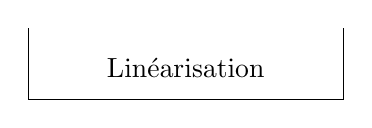
\begin{tikzpicture}\node at (2,0.4) {Linéarisation};\draw (0,.9)--(0,0)--(4,0)--(4,.9);\end{tikzpicture}}

$L\in\mathrm{Ob}\widehat A_{ab}$

On dit que $L$ est lisse si $\forall a\longrightarrow b$ dans $A$,
\diagram{\begin{tikzcd}[row sep=small]
\displaystyle\int_{A_a}L_a \arrow[r] \arrow[d,phantom,"\wr"] & \displaystyle\int_{A_b}L_b \arrow[d,phantom,"\wr"] \\
\displaystyle\int_A L^{(a)} \arrow[d,phantom,"\wr"] & \displaystyle\int_A L^{(b)} \arrow[d,phantom,"\wr"] \\
L^{(a)}*L_\bullet^{A^\circ} & L^{(b)}*L_\bullet^{A^\circ}
\end{tikzcd}}
est un quasi-iso.

On dit que $L$ est \uline{négligeable} si $L^{\unsure{b|\flat}}$ est quasi $=0$ (``quasi-nul'')

i.e. si $\displaystyle\int_{A_a}L=\int_A L^{(a)}$ est \uline{quasi-nul} pour tt $a$ de $A$.

\margin{Soit donc $L^{\unsure{b|\flat}}=(a\longmapsto L^{(a)}*L_\bullet^{A^\circ})$ dans $D_\bullet(\widehat B_{ab})$ c'est un complexe de chaînes dans $\widehat B_{ab}$ qui est \unsure{coh.}$^{\unsure{t}}$ loc.$^t$ constant, i.e. un ``\uline{syst. de coeff tordus}''.}

\margin{\unsure{p-iso} $L\longrightarrow L'$}

Soit \deleted{$\unsure{W}\,\unsure{\widehat A}$} $Lisse_{\mathbb Z}(A)$ la sous-cat pleine de $\widehat A_{ab}$ formée des objets lisses,

\margin{Lisse}

\textcircled{1} $\deleted{Lisse}\,W_{\unsure{q}}^{-1}Lisse_{\mathbb Z}(A)\longrightarrow D_\bullet^{l.c.}(\widehat B_{ab})$ \uline{est-ce une équivalence de catégories} ?

\diagram{\begin{tikzcd}[row sep=small]
D_\bullet^{l.c.}(\widehat B_{ab}) \arrow[d,phantom,"\unsure{\wr|?}"] \\
D_\bullet^{l.c.}(\widehat A_{ab}) \arrow[d,phantom,"\wr"] \\
\left[D_\bullet(Ab)\simeq Hot_{ab}\quad\text{si }A\text{ est asphérique}\right]
\end{tikzcd}}
\margin{par Quillen, peut se définir aussi comme $M_\bullet\longmapsto M_\bullet^{\unsure{b|\flat}}$}

\margin{OK pour $A=\Delta$, mais est-ce OK pour $A=\Delta_{/X}$, où $X\in\mathrm{Ob}\widehat\Delta$ ?}
\margin{$M_\bullet$}

\margin{\uline{NB} Si $A$ est tot. asph., \unsure{alors} \unsure{tous} les \unsure{pt} de $\widehat A_{ab}$ \unsure{quasi iso}}

\textcircled{2} Si $L,M$ dans $Lisse_{\mathbb Z}(A)$, a-t-on
\[
\mathrm{Ext}_{\mathbb Z_A}^i(L,M)\longrightarrow
\mathrm{Ext}_{\mathbb Z_B}^i(L^{\unsure{b|\flat}},M^{\unsure{b|\flat}})
\qquad\text{pour }i>0
\]
\margin{$\left[\simeq\mathrm{Ext}_{\mathbb Z}^i\left(\int_A L,\int_A M\right)\text{ si }A\text{ asph}\right.$}

[serait-ce vrai même sans supposer $L,M$ lisses ? \inserted{et peut-on y remplacer $L,M$ par $L_\bullet,M_\bullet$ ?}]

\textcircled{3} Supposons $L$ lisse, \deleted{et $H_i(L^{\unsure{b|\flat}})=0$ pour $i<N$. On cherche un $L'$,}
\inserted{et $N\in\mathbb N$. On cherche $L'\in\mathrm{Ob}\widehat A_{ab}$ et}
$L\longrightarrow L'$, tel que $L^{\unsure{b|\flat}}\longrightarrow L'^{\unsure{b|\flat}}$ identifie $L'^{\unsure{b|\flat}}$ au tronqué \inserted{homotopiq.} de $L^{\unsure{b|\flat}}$ en degrés $\unsure{\le|<}N$
